% % Chapter 2: XAFS Simulations
% % Chapter 2: XANES
% \textit{In this section, I can write about XANES to a super in-depth extent, and likely the bulk of this chapter will be about FEFF and FDMNES theoretical calculations}
% \section{Maybe derivation of EXAFS Equation}
% \section{FEFF vs. FDMNES Approaches}
% \section{Theoretical XANES Calculations}
% -------------------------------------------------------------

Before making any predictions, neural networks must first be trained on a large quantity of data. Specifically, to teach our neural network to predict the mean squared displacement (MSD)\textit{Of just Au NPs? Can we generalize this to the sigma of the PRDF?}, we must first generate a large quantity of training data comprised of XANES spectra, each labeled with a known MSD. Gathering such a large quantity of high-quality experimental data would be impractically time-intensitive and expensive. Rather, simulations provide a practical alternative, though even simulating each possible disordered structure individually, would be extremely time-intensive. Instead, we run many XANES simulations of simple, non-disordered structures and generate the neural network training data or disordered spectra via clever statistical averaging. In this chapter, we explain this statistical weighting process in-depth, beginning with the creation of simple, non-disordered spectra for the FEFF input files and culminating in the creation of many possible disordered spectra with known MSD.
\textit{Maybe give a brief outline of the process so you can understand the point of the sections as a walk-through before the very end}

\section{Generating Distortion Not Disorder}
Instead of creating structures with a range of \textit{disorder}, we instead begin by generating structures with a range of \textit{distortion}. Wheres \textit{disorder} refers to a statistical average of atomic displacement from their original position, characterized by MSD and the width $ \sigma^2 $ of a partial radial distribution function, \textit{distortion} refers only to isotropic expansion or contraction of the subject. Equivalently, we define distortion as a radial shift in all atomic positions away from (or towards) the center atomic absorber.

% Figure created in distortion-visualizations.ipynb 
\begin{figure}[h]
	\centering
	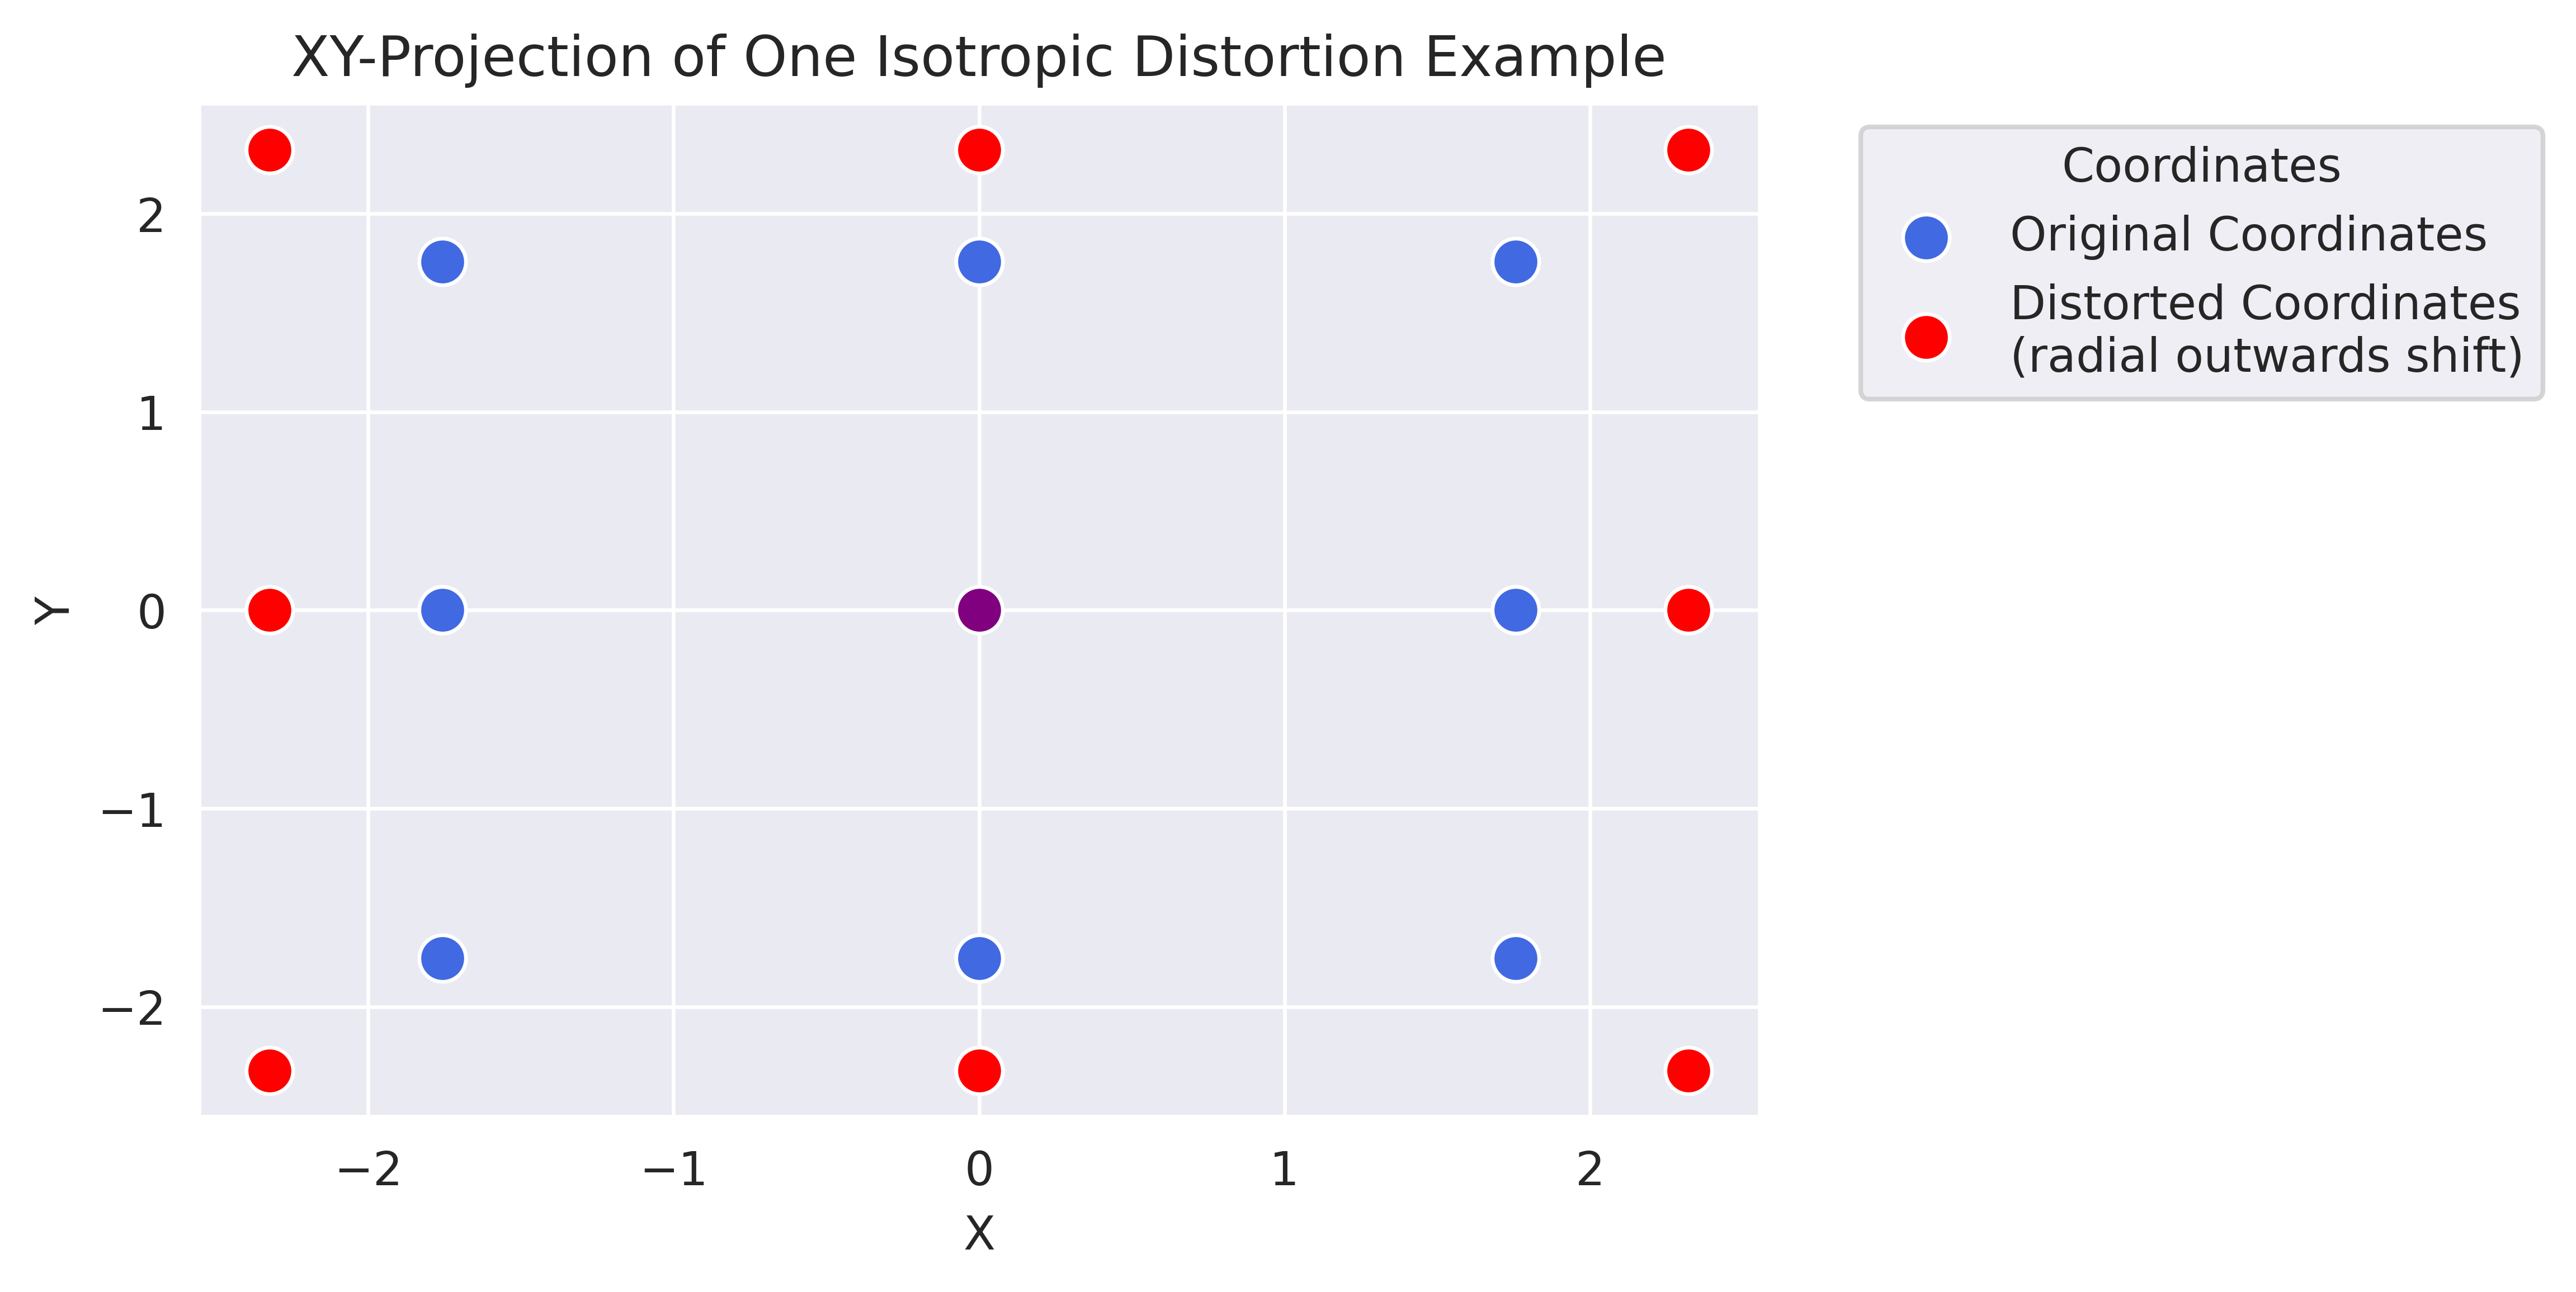
\includegraphics[width=\linewidth]{Chapters/Figures/2d_distortion_example.png}
	\caption[2D Distortion]{Each point represents an atom of first 12 nearest neighbors of a Au cluster projected onto the $xy$\nobreakdash-plane. The four corner points actually represent two atoms because of the projection. The blue atoms represent the original coordinates, and the red atoms represent the radially shifted coordinates. The center absorber atom is purple since its original position is the same as its distorted position.}
	\label{fig:2d-distortion}
\end{figure}

A 2-dimensional projection of this isotropic distorion is presented in Figure \ref{fig:2d-distortion}. Though the figure only shows the $xy$\nobreakdash-plane projection of the first 12 nearest neighbors, the actual structure used consists of the first four shells (55 atoms) with a lattice constant of 
4.0782~\AA~to match that of bulk Au.\textit{Citation? Wolfram Element Data?} In reality, the nearest-neighbor distances for Au nanoparticles are likely smaller \textit{citations?}; this can be accounted for later on in the averaging process since the original coordinates will only be one structure out of many. The important part is that the crystal structure is correct. 

We generate a total of 91 FEFF input files with different levels of distortion. Each file contains the same center absorber located at $ (0,0,0) $, but all other atomic coordinates are in a shifted location on the range of $ -0.45 $~\AA~to~$ +0.45 $~\AA~in increments of $ 0.01 $~\AA. For example, the FEFF input file with the greatest inward shift has all coordinates shifted $ 0.45 $~\AA~radially inwards towards the center absorber, and the FEFF input file with the largest outwards shift has coordinates shifted $ 0.45 $~\AA~radially outwards away from the center absorber.

\begin{minipage}{\linewidth}
Each FEFF input file is run with the following parameters: 
\begin{Verbatim}[samepage=true, numbers=left]
    SCF 4.6 0 30 .5 1
    EDGE    L3
    EXCHANGE    5   0.2 0.5
    S02 1.
    XANES   3.7 0.05    0.1
    FMS 7

    POTENTIALS
    0	79	Au	-1	-1	0.
    1	79	Au	-1	-1	0.
\end{Verbatim}
~
\end{minipage}

Running the 91 simulations (one for each of the distorted structure) takes approximately 30 minutues. Were we to generate thousands more or employ RMC or MD, this process could take weeks of compute time. We plot the resulting XANES spectra from the FEFF simulations in figure \ref{fig:feff-results}.

\begin{figure}[h]
	\centering
    \makebox[\textwidth][c]{
	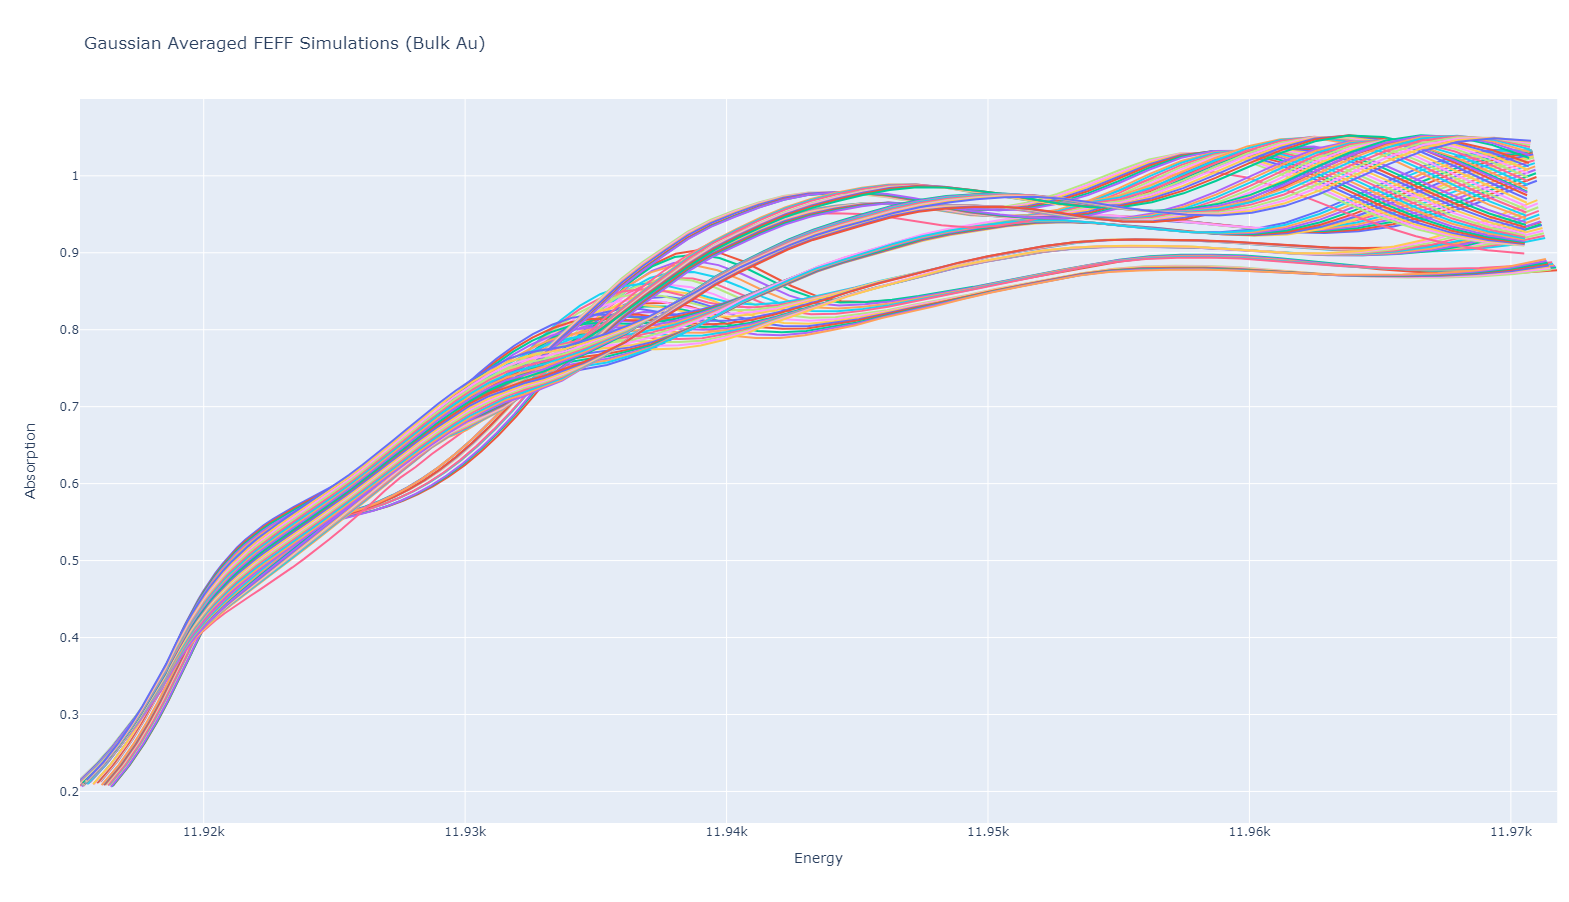
\includegraphics[width=1.1\linewidth]{Chapters/Figures/newplot.png}}
	\caption[FEFF Simulations Results]{\textit{TEMPORARY - way too much info. I'll select a few. }Each spectrum represents the FEFF simulation results for a different distorted structure. For each spectrum, the crystal structure and center absorber remain constant, the only parameter that varies is the euclidean distance from the center to the other coordinates.}
	\label{fig:feff-results}
\end{figure}

\section{Generating Disorder via Probability Distribution Averaging}

One way to characterize system disorder is with the Gaussian width, $ \sigma $ , of the partial radial distribution function. The idea of our statistical averaging method is to emulate this width by weighting the simulated XANES spectra accordingly. For example, Figure \ref{fig:gaussian-weighting-hist} depicts a histogram with $ \sigma=0.1 $~\AA. Each histogram bin represents a simulated XANES spectrum with a different isotropic displacement. For example, the bin at $ \Delta\rho=0.0 $~\AA~represents the simulated XANES spectrum with no distortion, and the bin at $ \Delta\rho=-0.2 $~\AA~represents the simulated XANES spectrum with all the atomic coordinates shifted isotropically inwards towards the center absorber by $ 0.2 $~\AA. The height of each bin, $ f(\Delta\rho) $, represents the relative contribution of each simulated XANES spectrum towards the resulting weighted spectrum. For visual clarity, Figure \ref{fig:gaussian-weighting-hist} depicts only 40 bins; the actual weighting includes 91 bins ranging from $ -0.45 $~\AA~to~$ +0.45 $~\AA.
% figure created in playground.ipynb
% !htb
\begin{figure}[h!]
	\centering
	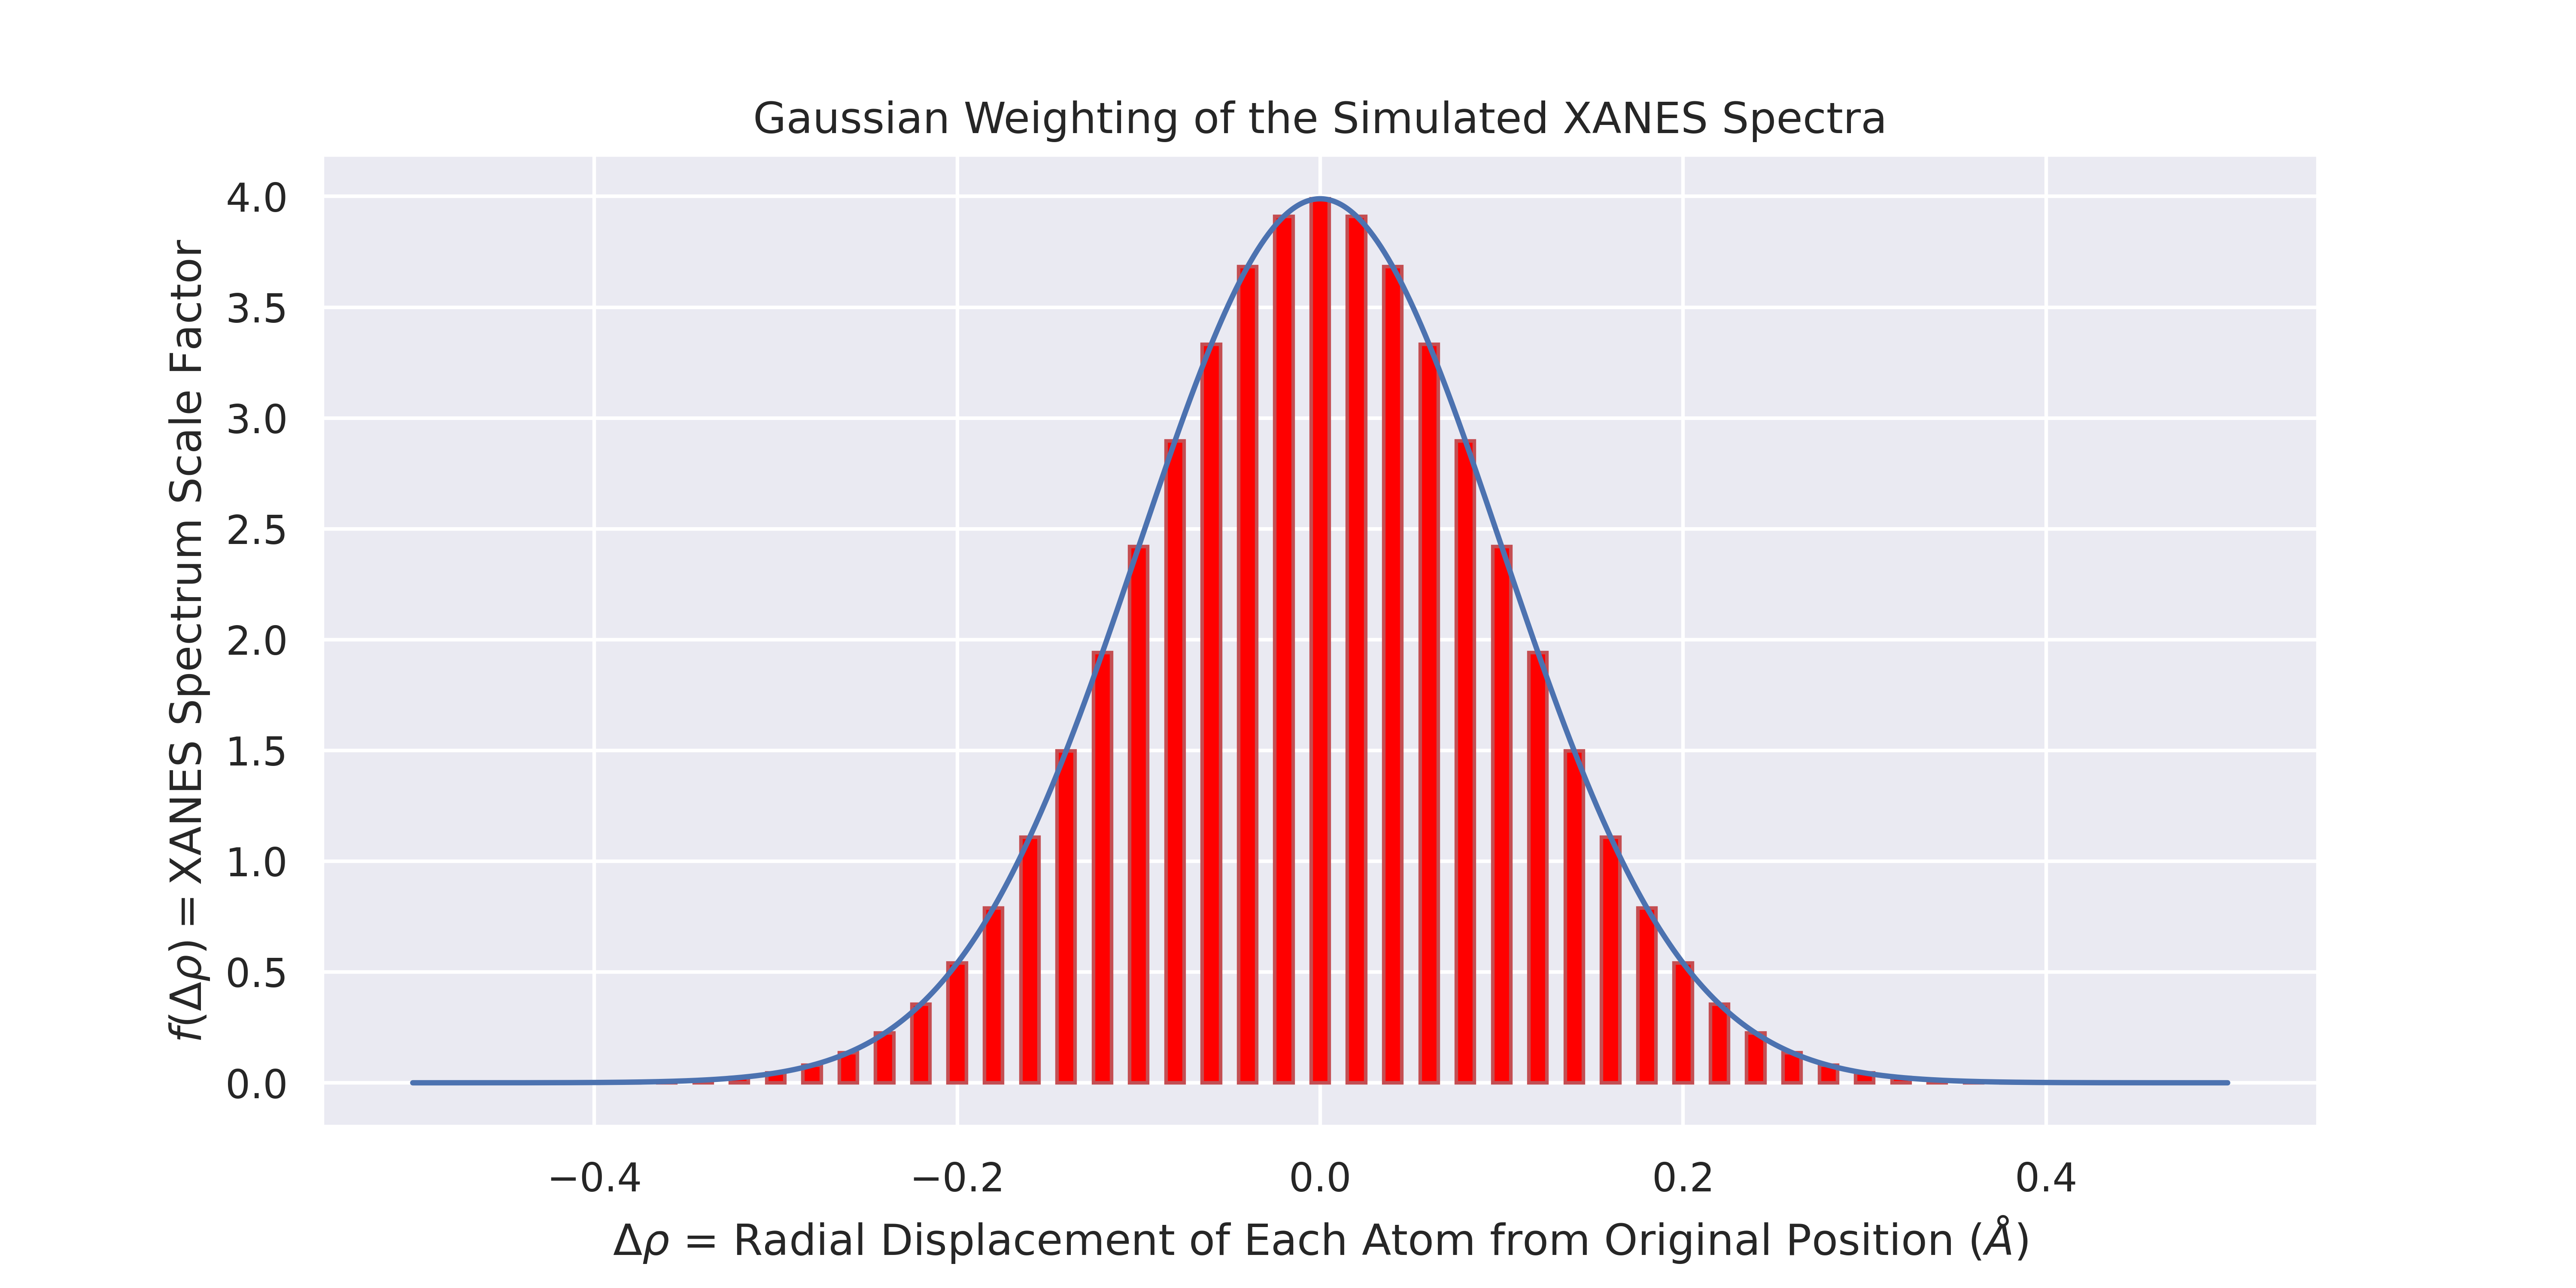
\includegraphics[width=\linewidth]{Chapters/Figures/gaussian-weighting-hist.png}
	\caption[Simulated Spectrum Gaussian Weighting]{A Gaussian distribution probability density function can be used to calculate the relative weight of each FEFF generated XANES spectrum towards one simulated, disordered spectrum. Each bin (red bar) represents a FEFF generated spectrum; the $x$-axis is the isotropic shift of the atomic positions, and the $y$-axis is the relative weight factor.}
	\label{fig:gaussian-weighting-hist}
\end{figure}

The disordered, gaussian-averaged XANES spectrum, $ \left\langle \mu(E) \right\rangle $, using the histogram weighting of the gaussian in Figure \ref{fig:gaussian-weighting-hist} is calculate via Equation (\ref{eqn:gaussian-averaging}):

\begin{equation}
	\label{eqn:gaussian-averaging}
	\left\langle \mu(E) \right\rangle  = \frac{1}{S} \sum_{\Delta\rho=-.45}^{+.45} g\left(\Delta \rho \mid \mu=0, \sigma=0.1\right) \mu(E \mid \Delta\rho)
\end{equation}

\noindent
In the above equation, $ \Delta\rho $ is the isotropic, radial displacement of each atom from its original position, and $ \mu(E \mid \Delta\rho) $ is the simulated FEFF spectrum for the given $ \Delta\rho $ configuration. Furthermore, in Equation (\ref{eqn:gaussian-averaging}), $ S $ represents a standardization factor needed to negate the effect of the changing Gaussian height as a function of the variance, $ \sigma^2 $. With the inclusion of $ S $ , only the relative heights of each bin matters for producing the averaged XANES spectrum. This standardization factor is defined in Eqation (\ref{eqn:gaussian-standardization}):

\begin{equation}
	\label{eqn:gaussian-standardization}
	S = \sum_{\Delta\rho=-.45}^{+.45} g\left(\Delta \rho \mid \mu=0, \sigma=0.01\right)
\end{equation}

\noindent
In both equations (\ref{eqn:gaussian-averaging}) and (\ref{eqn:gaussian-standardization}), the function $ g $ is just the typical Gaussian distribution probability density function (Equation \ref{eqn:gaussian}): 

\begin{equation}
	\label{eqn:gaussian}
	g(x) = \frac{1}{{\sigma \sqrt {2\pi } }}e^{{{ - \left( {x - \mu } \right)^2 } \mathord{\left/ {\vphantom {{ - \left( {x - \mu } \right)^2 } {2\sigma ^2 }}} \right. \kern-\nulldelimiterspace} {2\sigma ^2 }}}
\end{equation}

The above example only generates one (simulated) disordered XANES spectrum and does so via weighting of a Gaussian distribution with mean and variance equal to $ 0 $ and $ 0.01 $, respectively. To simulate systems with different degrees of disorder, we can vary the shape of the probability density function. With a Gaussian distribution, we can only vary the mean and variance; to simulate even more conditions, however, we can instead use the multivariate skew-normal distribution (\ref{eqn:skew-norm}) \cite{skewnorm_Azzalini_1999, 2020SciPy-NMeth}, \textit{f(x)}.

\begin{equation}
	\label{eqn:skew-norm}
	f(x)=2\phi (x)\Phi (\alpha x)
\end{equation}
 
\noindent
where $ \phi(x) $ is the Gaussian PDF:
\begin{equation}
	\label{eqn:skew-norm-pdf}
	\phi (x)={\frac  {1}{{\sqrt  {2\pi }}}}e^{{-{\frac  {x^{2}}{2}}}}
\end{equation}

\noindent
and $ \Phi (x) $ is the Gaussian CDF:
\begin{equation}
	\label{eqn:skew-norm-cdf}
	\Phi (x)=\int _{{-\infty }}^{{x}}\phi (t)\ dt
\end{equation}

%------------WIKIPEDIA EQUATION VERSION -------------
% \begin{equation}
% 	\label{eqn:skew-norm-cdf}
% 	\Phi (x)=\int _{{-\infty }}^{{x}}\phi (t)\ dt={\frac  {1}{2}}\left[1+\operatorname {erf}\left({\frac  {x}{{\sqrt  {2}}}}\right)\right]
% \end{equation}
% \noindent
% and erf is Gauss' error-function

% \begin{equation}
% 	\label{eqn:skew-norm-cdf-erf}
% 	{\displaystyle \operatorname {erf} \left(z\right)={\frac {2}{\sqrt {\pi }}}\int _{0}^{z}e^{-t^{2}}\,dt}
% \end{equation}

\noindent
Equation (\ref{eqn:skew-norm}) includes the shape parameter, $ \alpha $, which has the nice property of producing a right-skewed distribution when positive and a left-skewed distibution when negative. When $ \alpha=0 $, the distribution simply produces the typical Gaussian distribution (eq. \ref{eqn:gaussian}). Utilizing equation (\ref{eqn:skew-norm}), we can vary $ \mu, \sigma,  $ and $ \alpha $ to alter the first four moments of the function: mean, standard deviation, skew, and kurtosis. Eighteen possible skew-norm weighting functions are plotted in Figure \ref{fig:skew-norm-options}. To produce the neural network training data, 1000 such weightings are used.

\begin{figure}[h!]
	\centering
	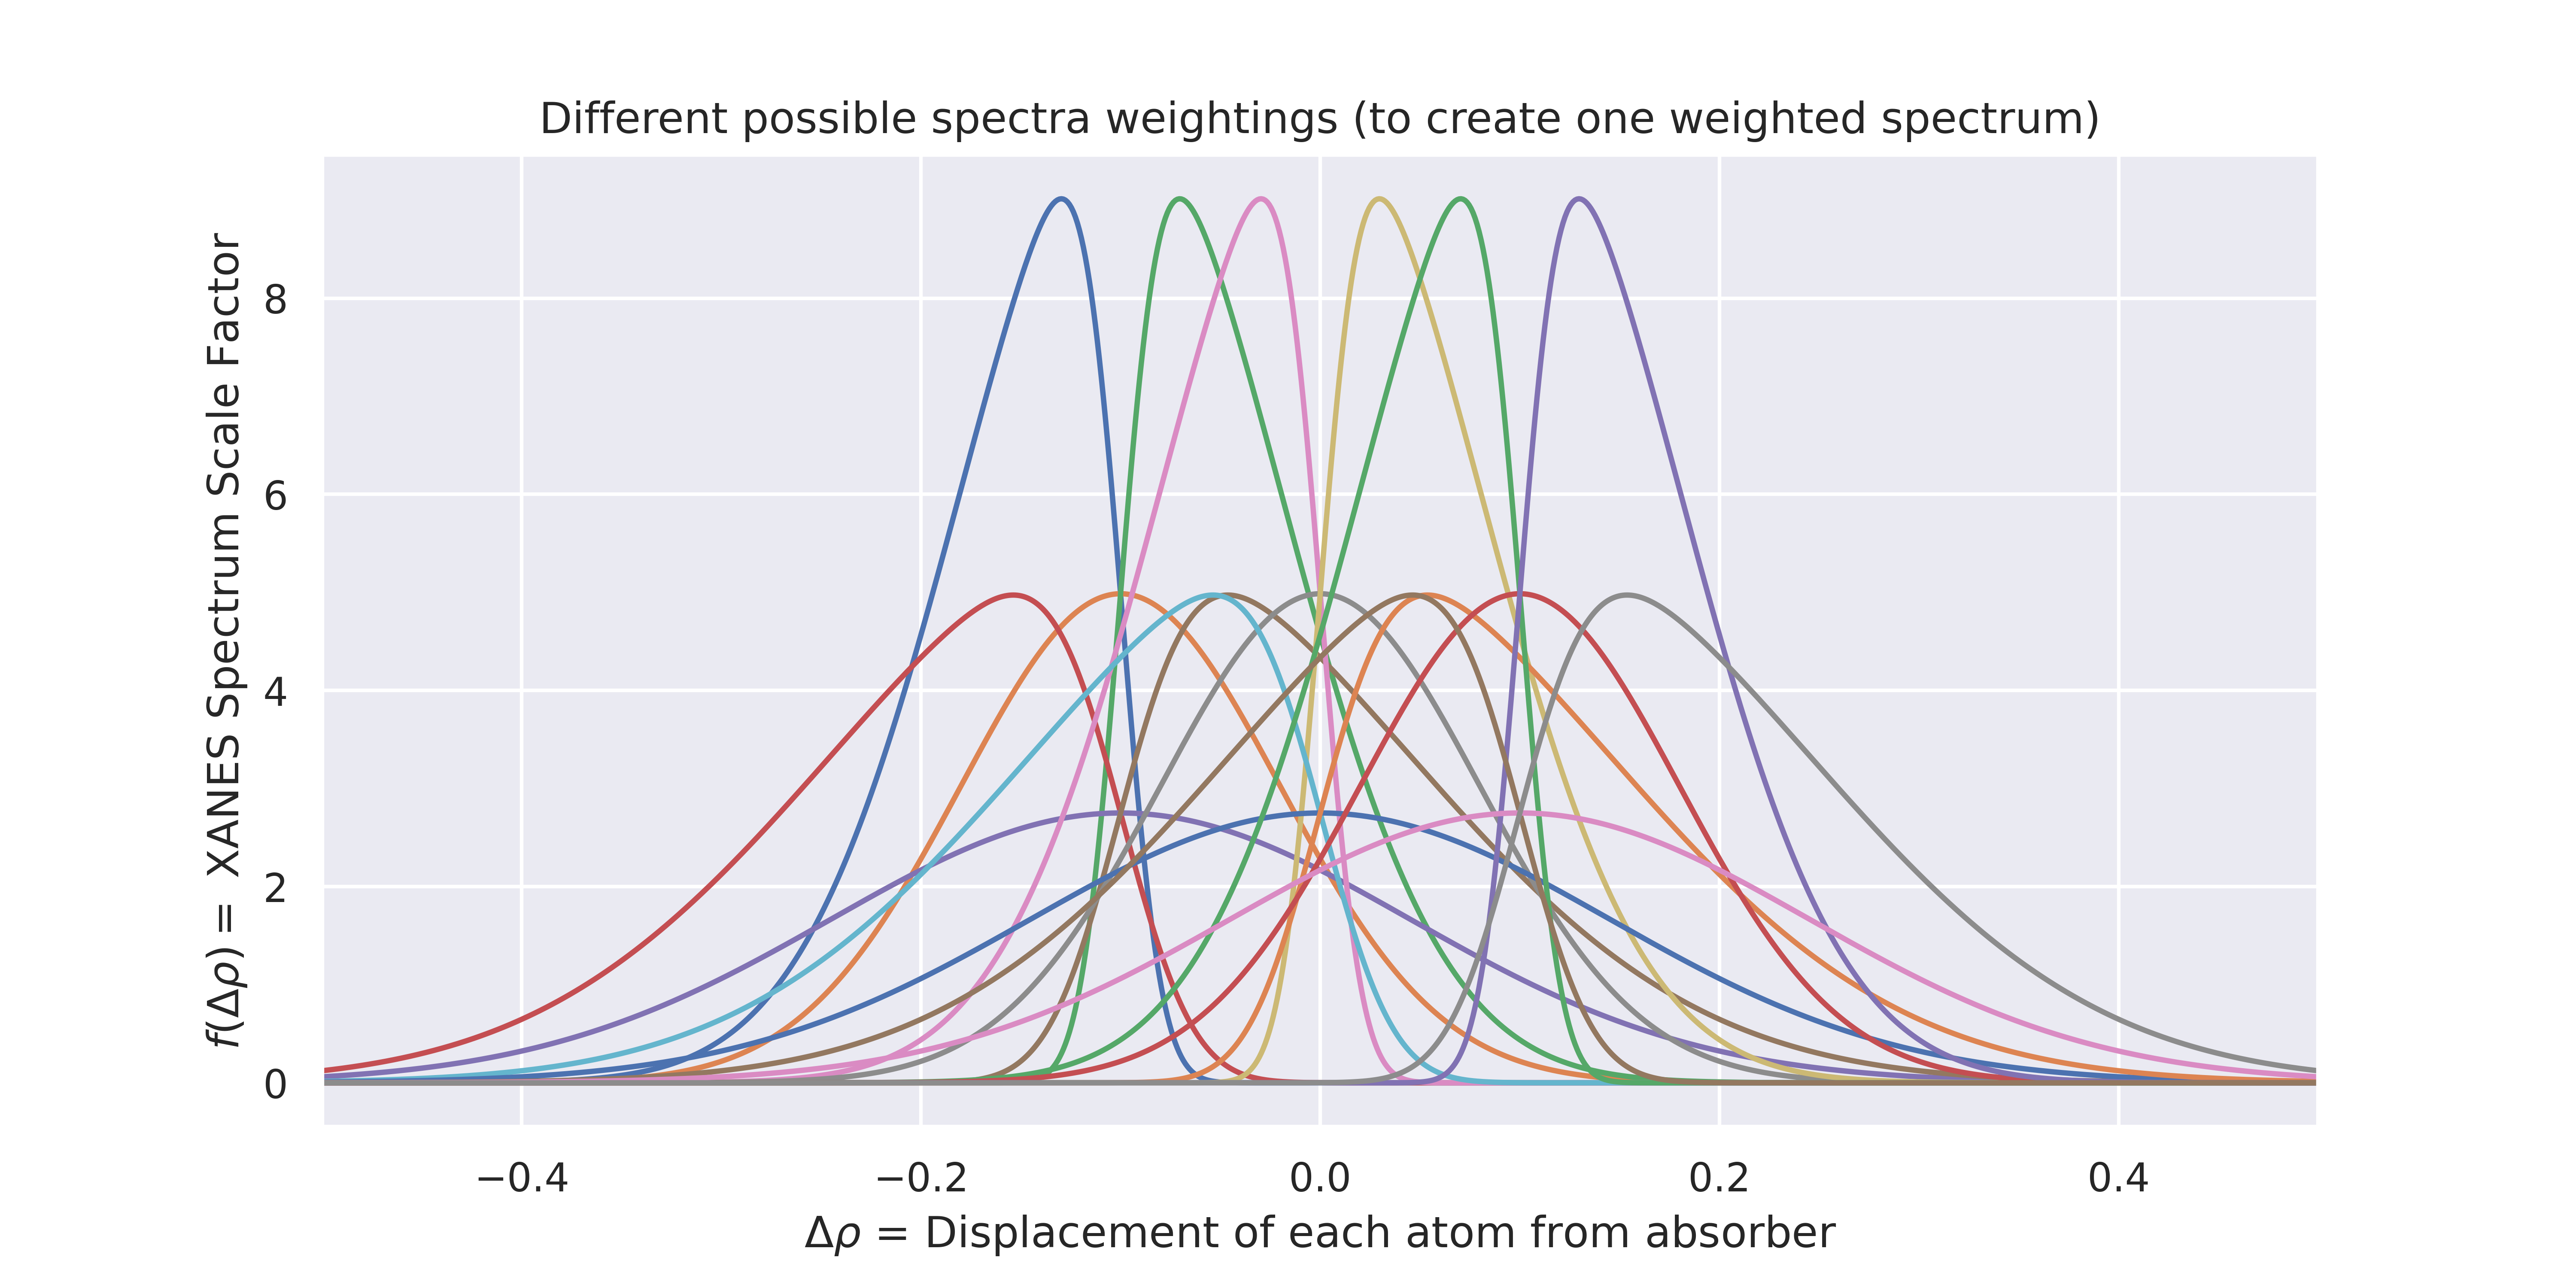
\includegraphics[width=\linewidth]{Chapters/Figures/skewnorm_options.png}
	\caption[Simulated Disordered Spectrum Weightings]{Eighteen skew-norm distributions plotted with all possible combinations of $ \sigma=\{.08, .145\} $, $ \mu=\{-.1, 0, .1\} $, and $ \alpha=\{-5,0,5\} $. Each represents a possible way to produce a simulated, disordered spectrum from many FEFF-simulated, distorted spectra} 
	\label{fig:skew-norm-options}
\end{figure}

The disorder of the skew-norm generated, disordered spectrum is characterized by the mean squared displacement of each atom from its original position ($ \Delta\rho $ ), weighted in the same manner as the spectra. \textit{Instead of characterizing the disordered spectrum by the standard deviation of the gaussian used to create it.} The weighted mean squared displacement, $ MSD $, is calculated via equation (\ref{eqn:weighted-MSD}):

\begin{equation}
	\label{eqn:weighted-MSD}
	MSD  = \frac{1}{S} \sum_{\Delta\rho=-.45}^{+.45} f\left(\Delta \rho \mid \mu, \sigma^2, \alpha \right) 
\end{equation}

\noindent
Here, $ f(x) $ is the skew-norm function from equation (\ref{eqn:skew-norm}), and the $ MSD $  of each individual FEFF spectrum is equal to the isotropic distortion, $ \Delta\rho $.  

\section{Simulation vs. Experimental Data}

To check our FEFF simulation parameters, as well as the validity of the gaussian-weighted disorder technique, we compare the simulation data to experimental data. \textit{Can someone give me citations for these?} In Figure \ref{fig:avg-experimental-vs-simulation}, both experimental and simulation spectra for bulk-like and nanoparticle scenarios are plotted. EXAFS fitting was used to characterize the disorder in the experimental measurements. For the bulk foil, this parameter was found to be $ \sigma^2=0.0081(5)~$ {\AA}$ ^2 $, and for the 8~nm disordered particle, $ \sigma^2=0.0102(8) $~{\AA}$ ^2 $.  One simulated, disordered spectrum was weighted according to the gaussian $ N(0, 0.09) $ to represent the disordered nanoparticle, and the other was weighted according to the gaussian $ N(0, 0.038)  $ to represent the bulk. These weightings correspond to $ MSD $ values that match the measured $ \sigma^2 $ values for the experimental data.  

\begin{figure}[h]
	\centering
	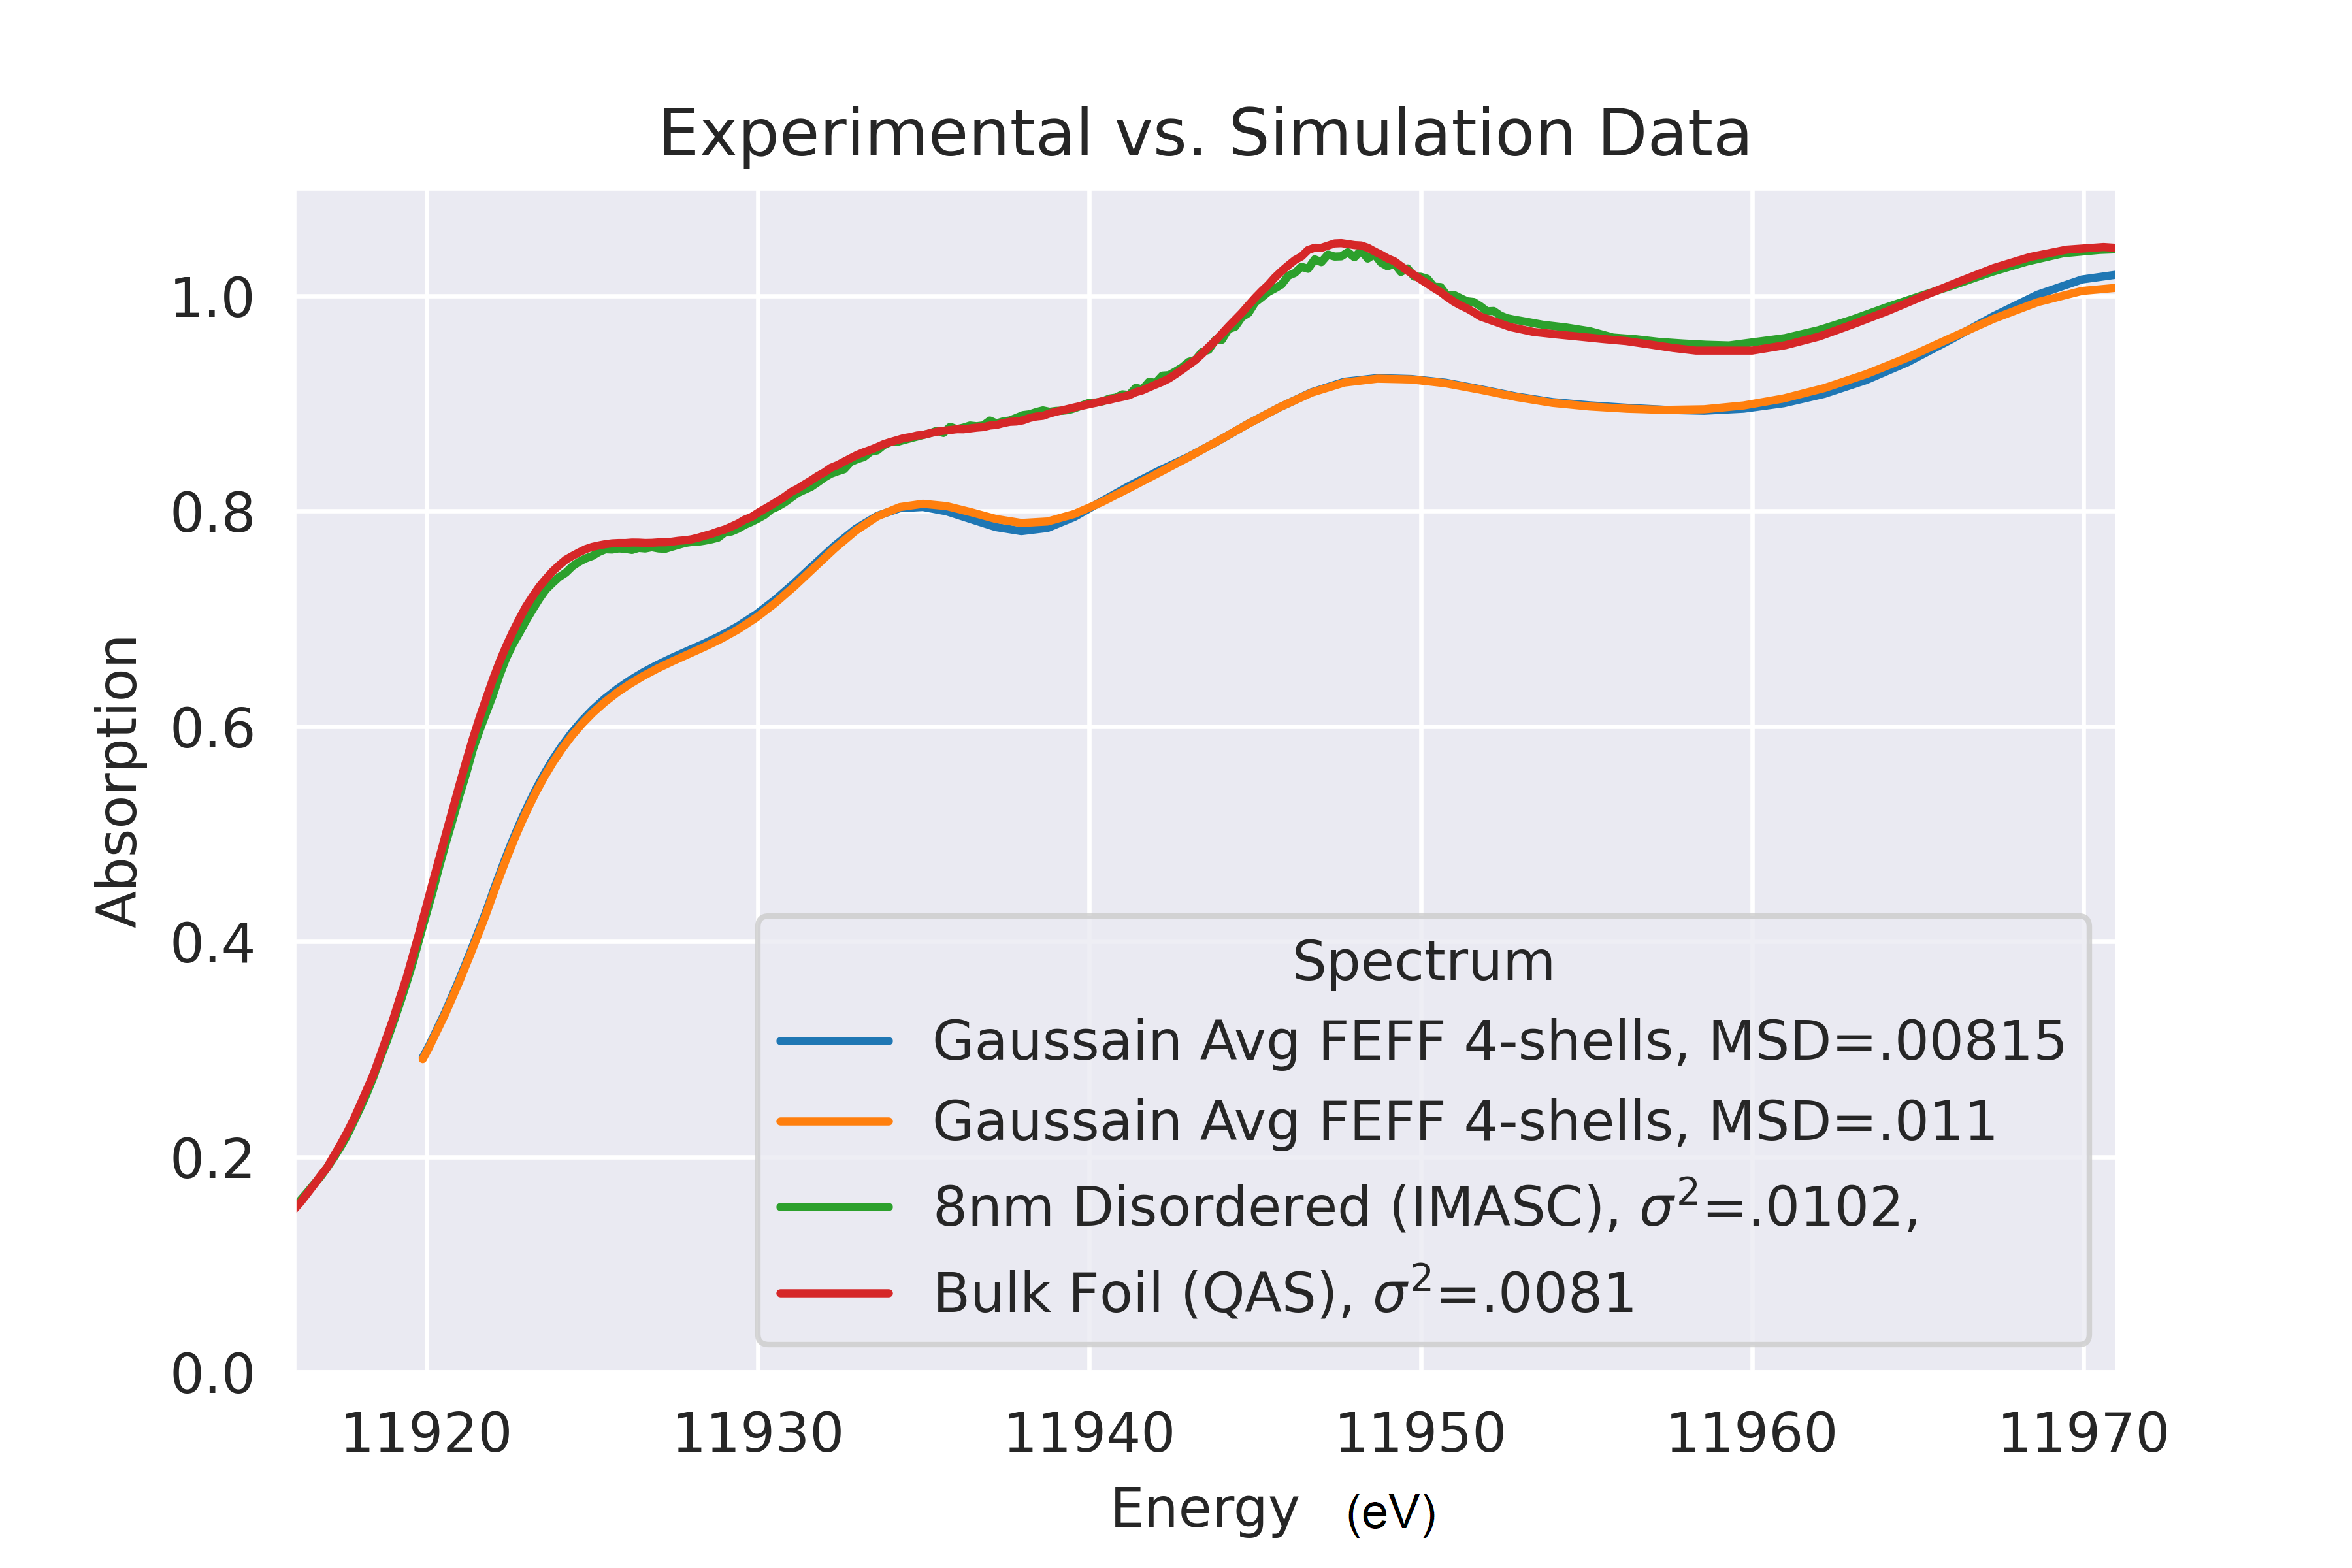
\includegraphics[width=.75\linewidth]{Chapters/Figures/updated_bulk_8nm_disorder_experimental_theory_comparison.png}
	\caption[Simulation vs. Experimental]{Comparing the bulk foil (red) measurement to the 8~nm disordered nanoparticle (green) measurement is an analog to comparing the simulated, non disordered FEFF spectrum (blue) to the simulated disordered spectrum (orange).}
	\label{fig:avg-experimental-vs-simulation}
\end{figure}

In Figure \ref{fig:avg-experimental-vs-simulation}, the bulk Au foil spectrum is above the 8~nm nanoparticle spectrum (more absorption) until the peak around 11937~eV, where the NP absorption becomes higher. The two criss-cross again over the next two peaks, changing which material has the higher absorbance in an energy range. This change is more easily seen in Figure \ref{fig:avg-experimential-vs-simulation-difference}, which plots the difference between the the bulk material and the nanoparticle absorption for both the experimental measurements and the simulations. The experimental and simulation difference-spectra follow the same trend with the exception of the peak around 11947~eV.
% The two spectrum switch again at the peak around 11943~eV so the bulk foil's absorption nlevel is higher again. Beyond this peak, the two


\begin{figure}[h!]
	\centering
	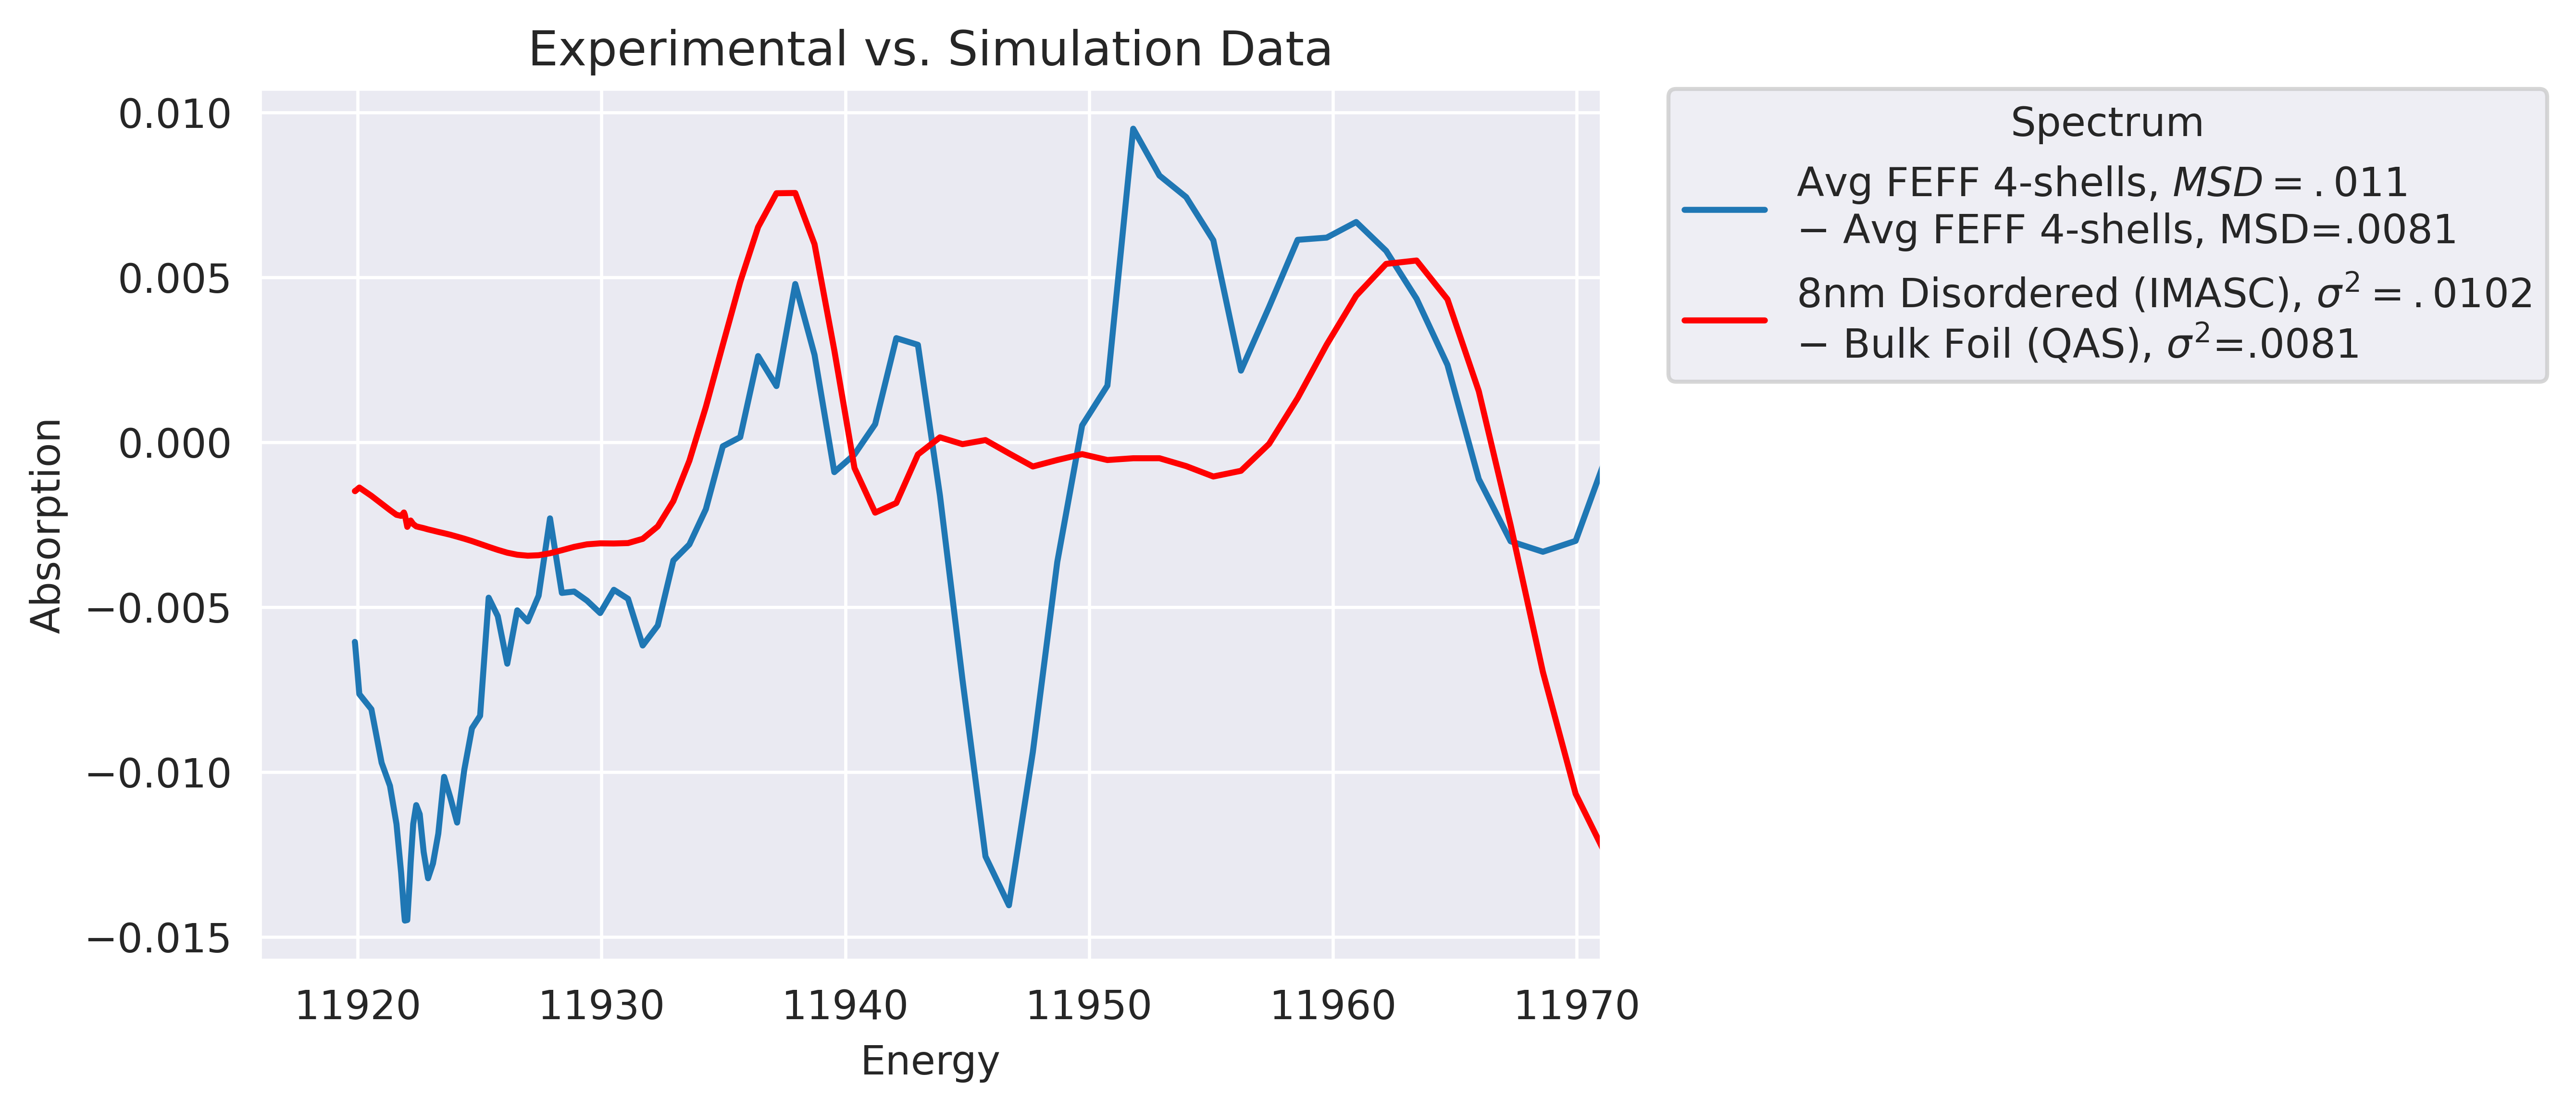
\includegraphics[width=\linewidth]{Chapters/Figures/experimental_vs_simulation_delta.png}
	\caption[Bulk-nanoparticle difference: Simulation vs. Experimental data]{The difference between the nanoparticle spectrum and the bulk spectrum are plotted for the same data as in Figure \ref{fig:avg-experimental-vs-simulation}. It is easier to see where the bulk and the nanoparticle absorption crisscross by plotting the difference.}
	\label{fig:avg-experimential-vs-simulation-difference}
\end{figure}

Figures \ref{fig:avg-experimental-vs-simulation} and \ref{fig:avg-experimential-vs-simulation-difference} aren't meant to be perfect comparisons of simulations vs. experimental data. For one, the experimental data compares a bulk spectrum to a nanoparticle. By contrast, both the simulation spectra are of the same size 55 atom cluster. Still, much of the disorder trends are coded in the simulation approach. 

To test if the size information is also coded in our simulations, we compare different size simulations to experimental data in Figure \ref{fig:avg-experimental-vs-simulation2}. As expected, including more atoms in the simulation produces more bulk-like spectrum characteristics, such as larger amplitude peaks.

\begin{figure}[h]
	\centering
	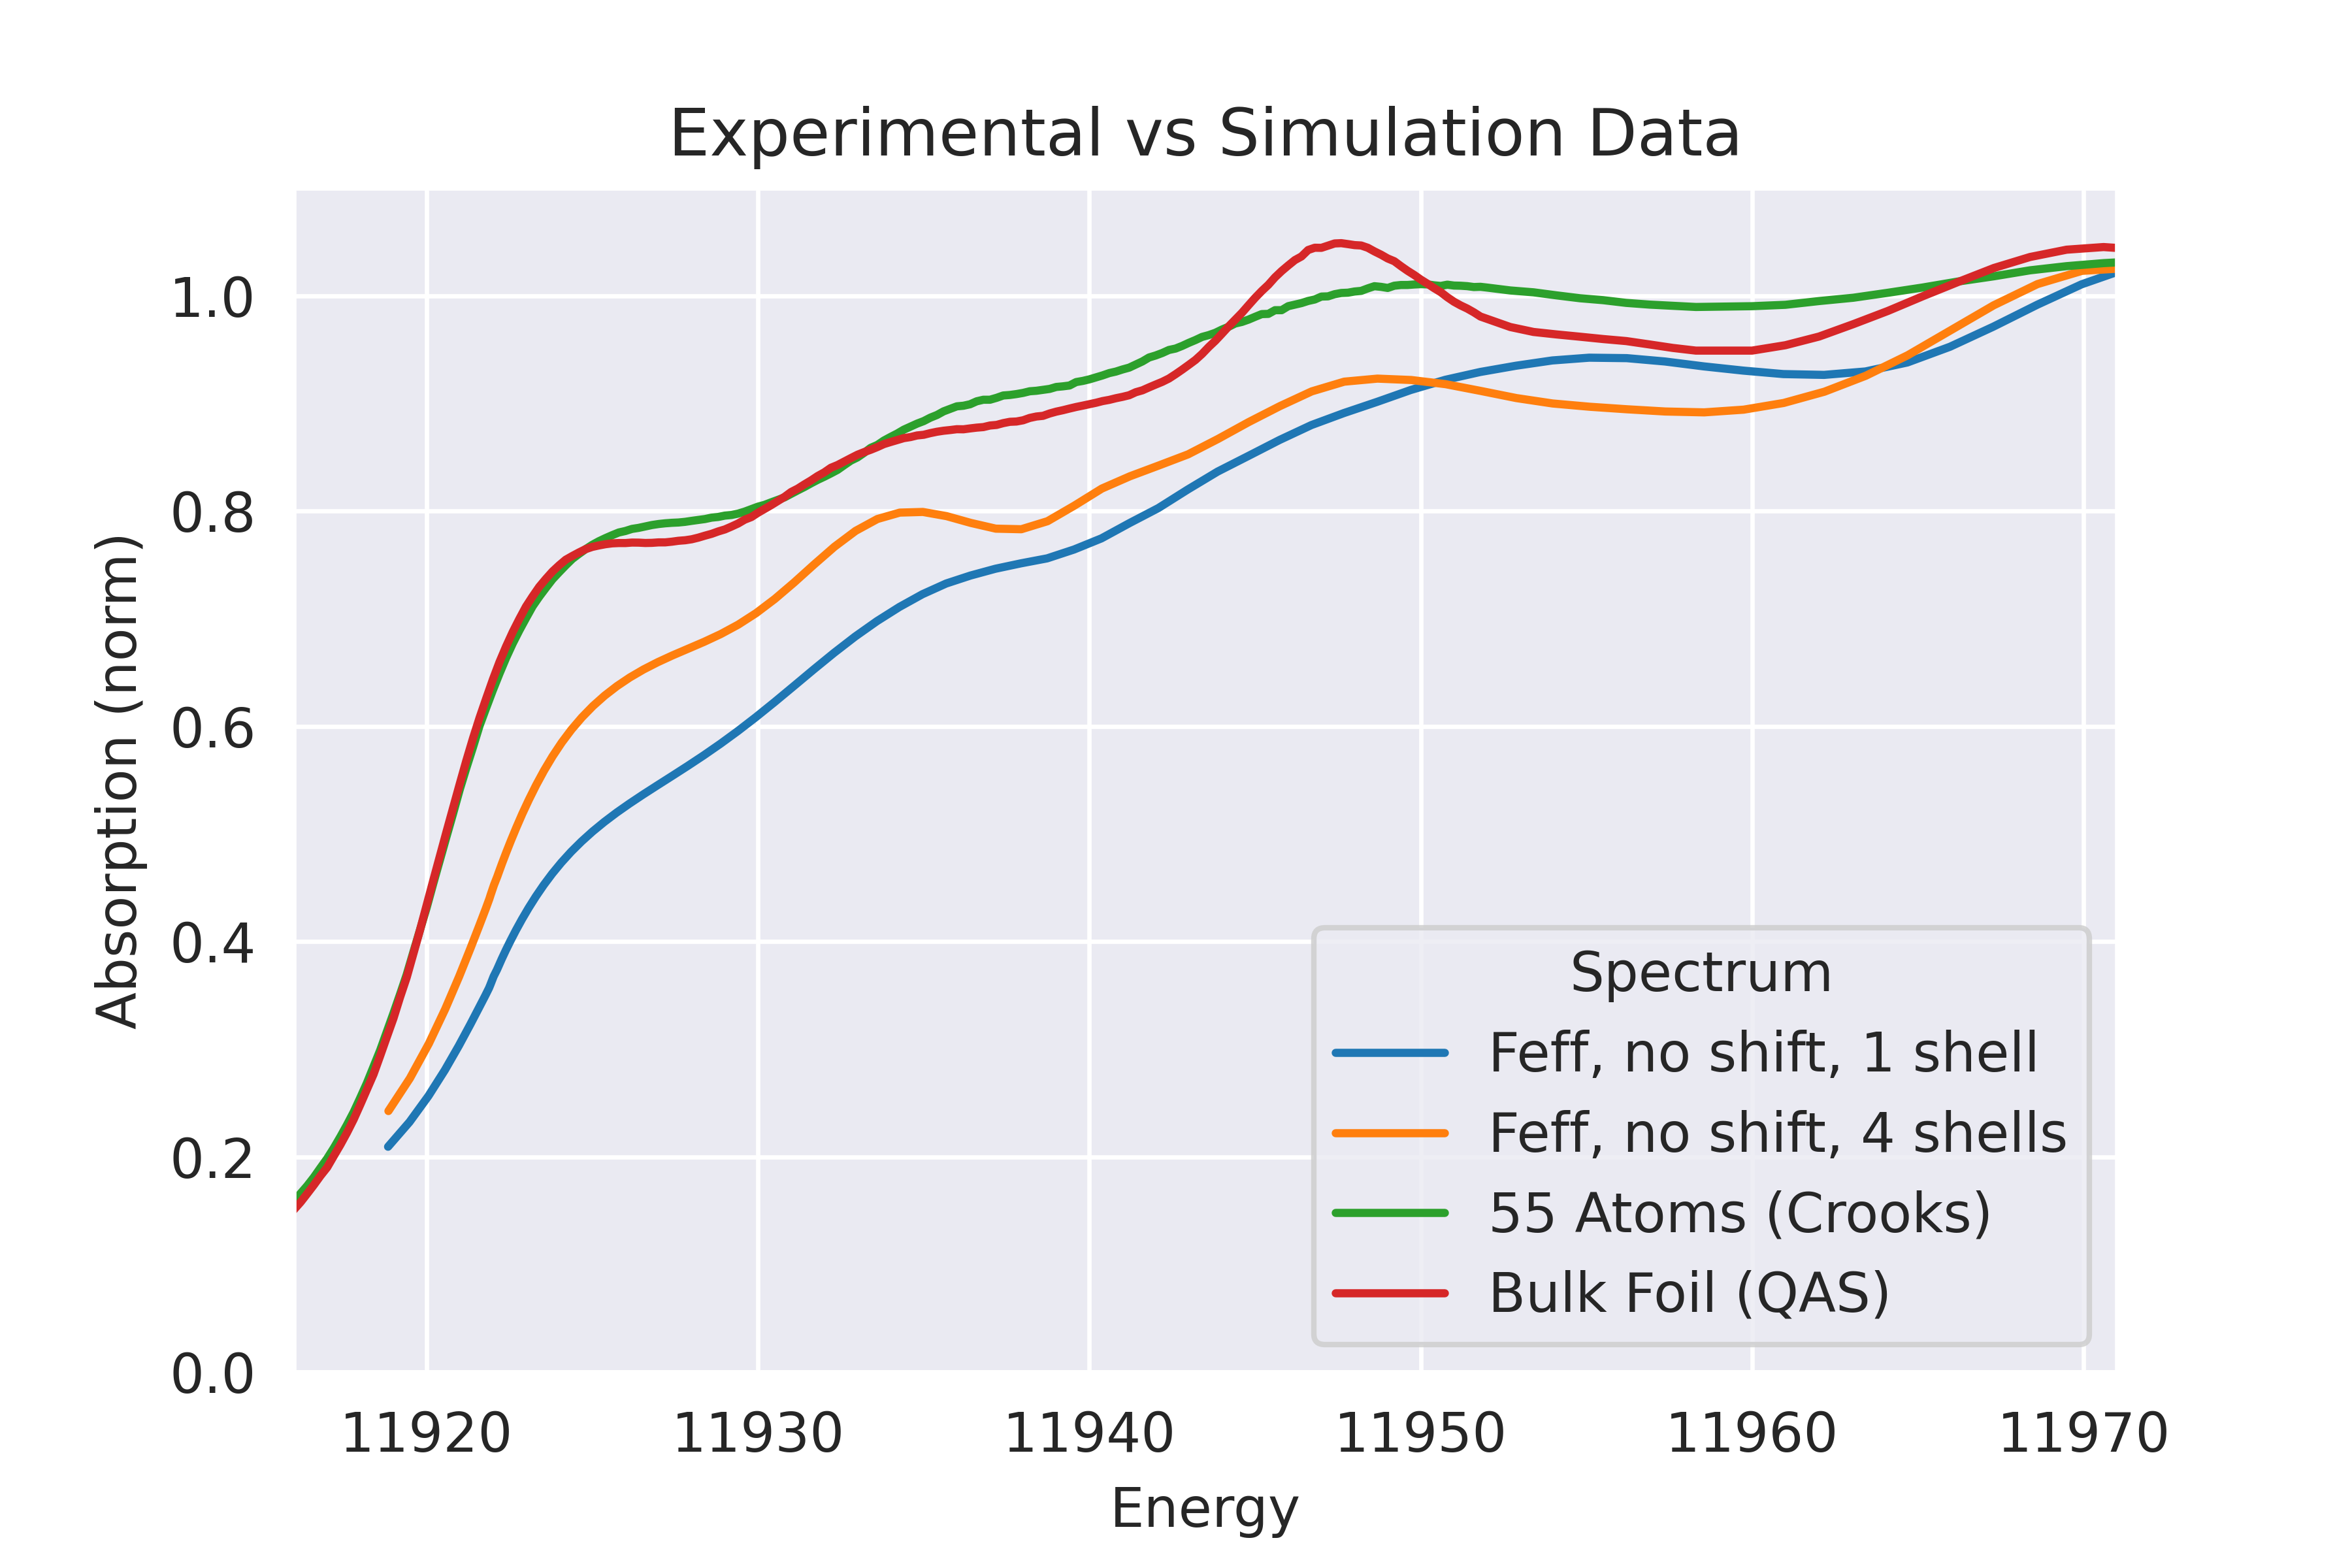
\includegraphics[width=.7\linewidth]{Chapters/Figures/Bulk_55atom_experimental_theory_comparison.png}
	\caption[Simulation vs. Experimental 2]{Comparing the bulk foil (red) measurement to the 55 atom nanoparticle (green) measurement is an analog to comparing the 13 atom simulated spectrum (blue) to the 55 atom simulated spectrum (orange).}
	\label{fig:avg-experimental-vs-simulation2}
\end{figure}

I NEED A PLOT COMPARING THIS METHOD TO PARTICLE AVERAGED METHOD HERE.

\section{Particle-Averaged FEFF Simulated Disordered Structures}

\begin{figure}[h]
	\centering
	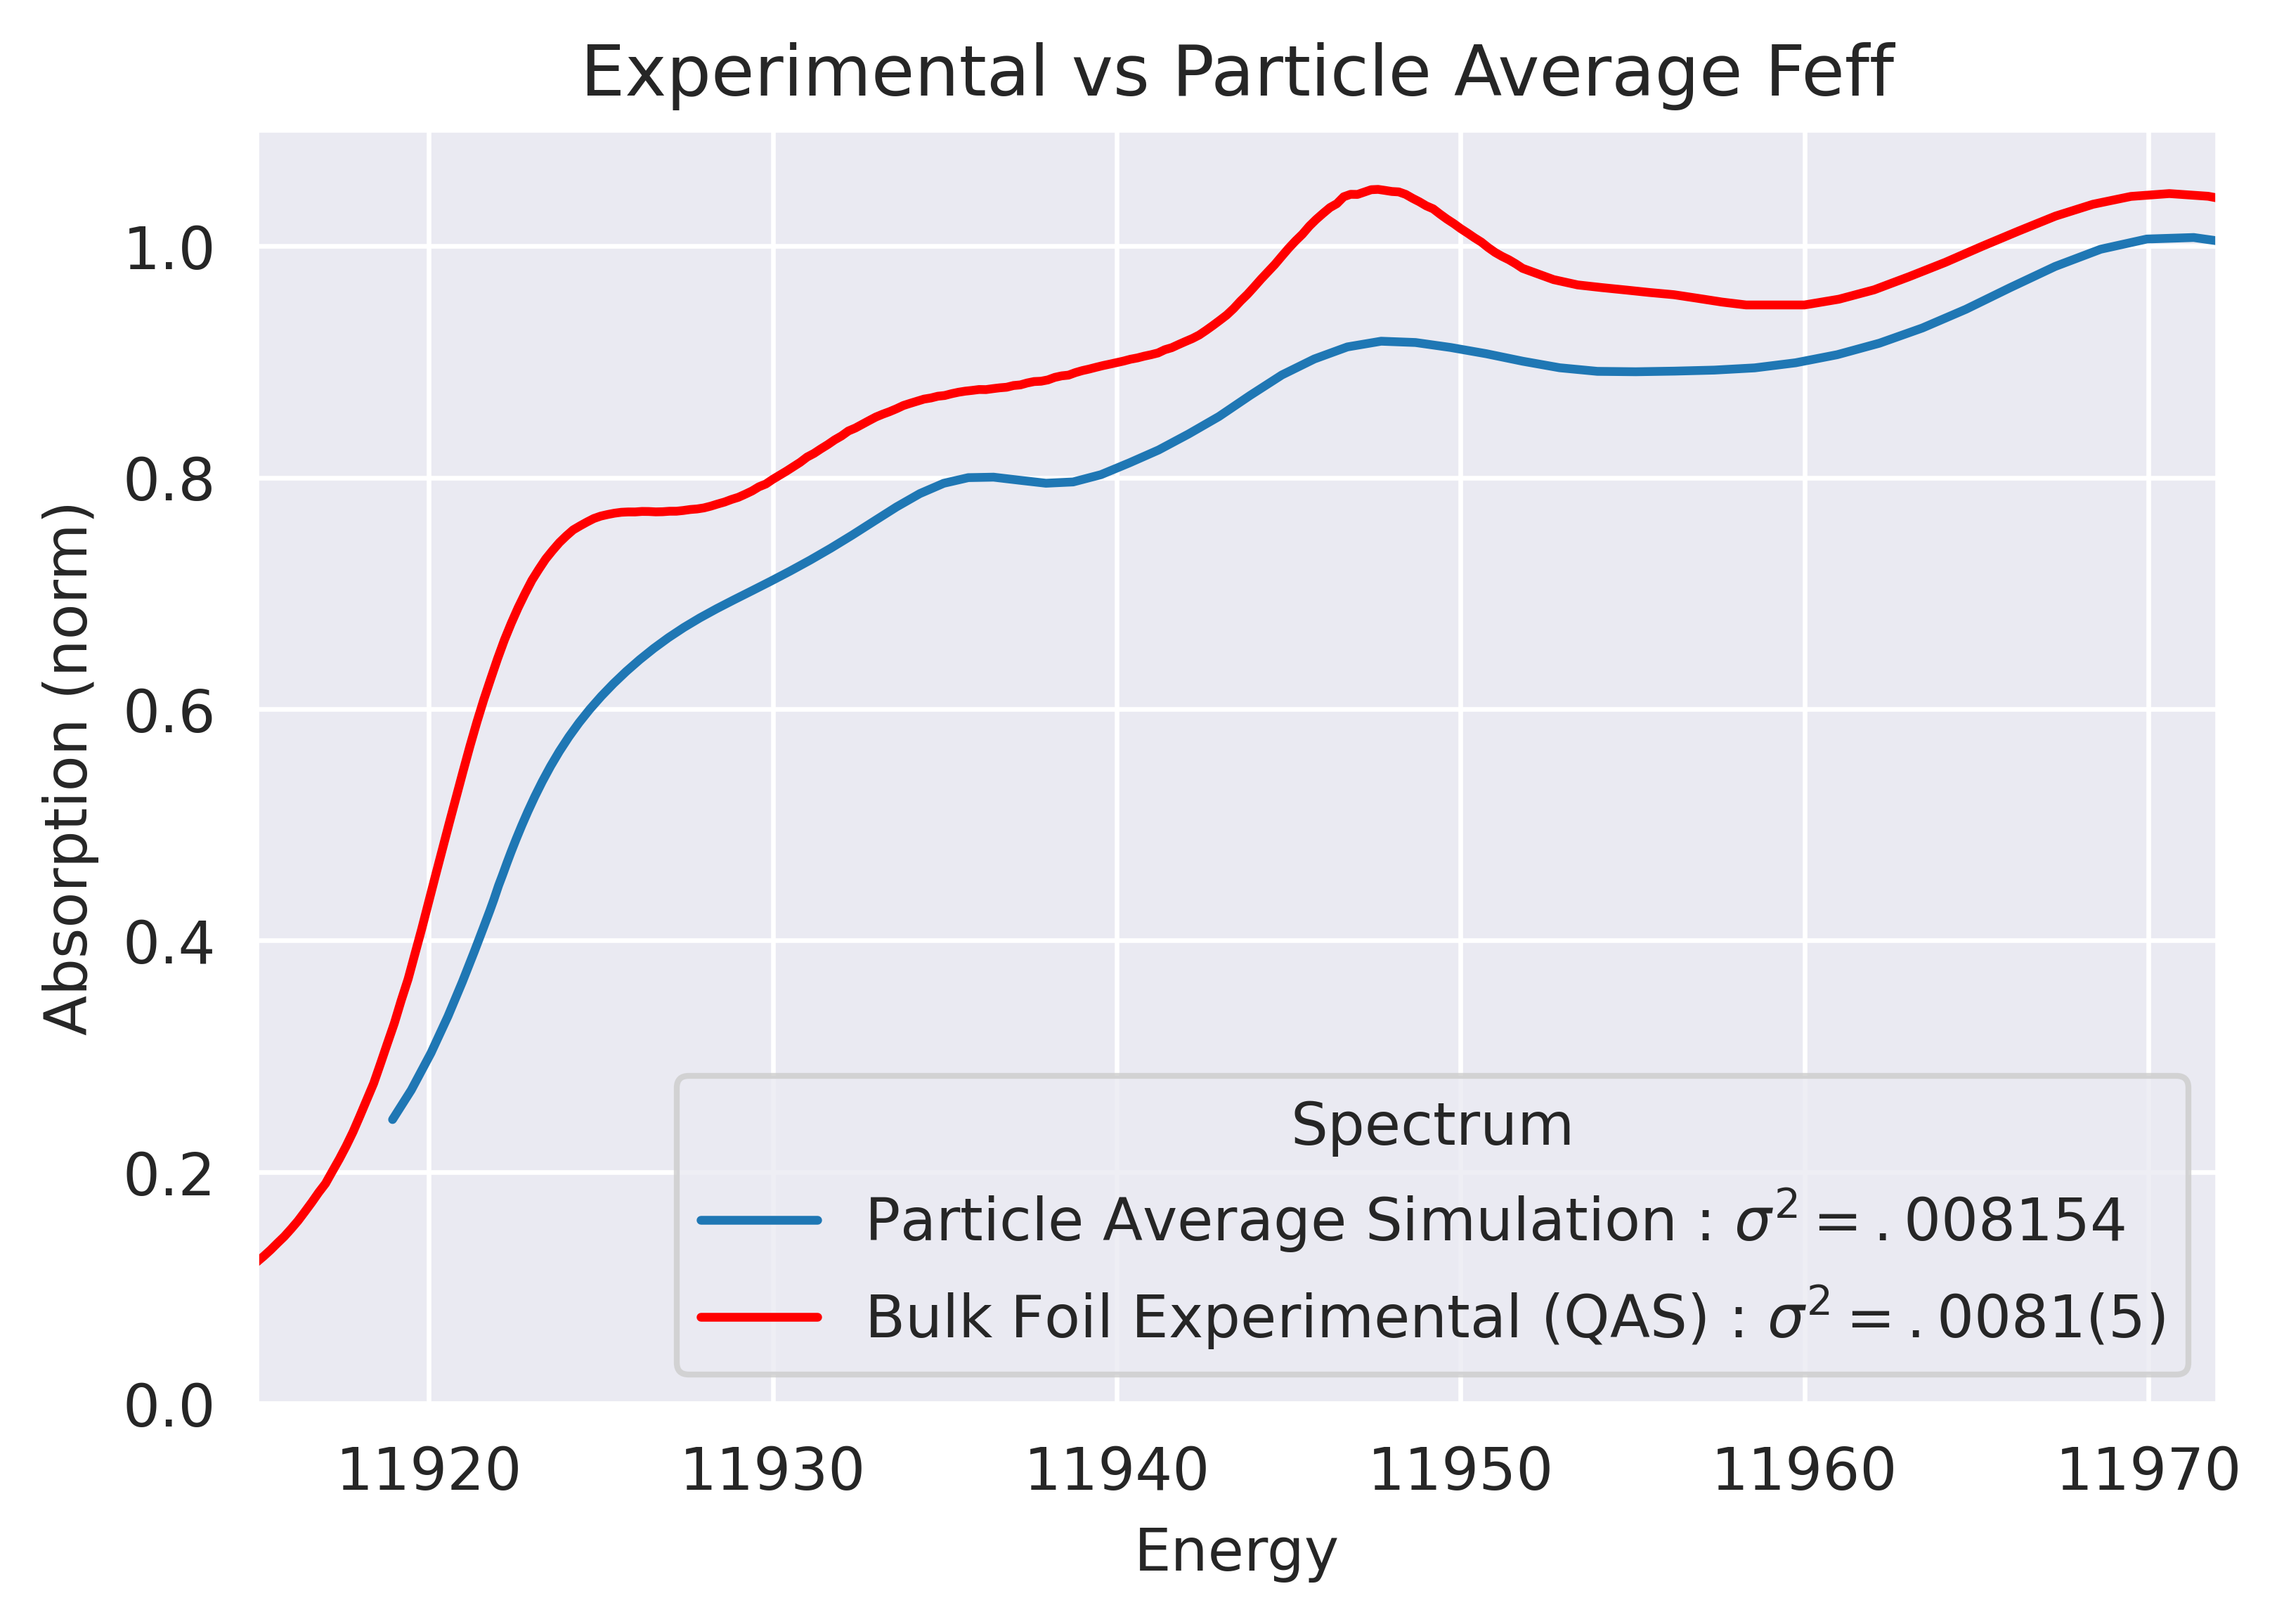
\includegraphics[width=.7\linewidth]{Chapters/Figures/Bulk_experimental_vs_pa_comparison.png}
	\caption[Simulation vs. Experimental 3]{Comparing the bulk foil (red) measurement to a simulated large, bulk-like nanoparticle with the same disorder. The FEFF-}
	\label{fig:avg-experimental-vs-simulation2}
\end{figure}

